\large{

\section{Struttura dati}
blablalba
\begin{figure}[!htb]
	\begin{center}
		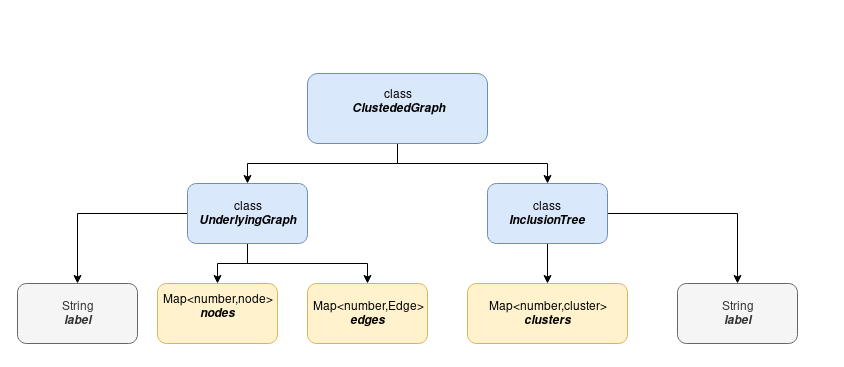
\includegraphics[width=1 \linewidth]{figure/cgraphClass}
	\end{center}
	\caption{Oggetto clusteredGraph\label{fig:cgraphClass}}
\end{figure}
blablalba
\begin{figure}[!htb]
	\begin{center}
		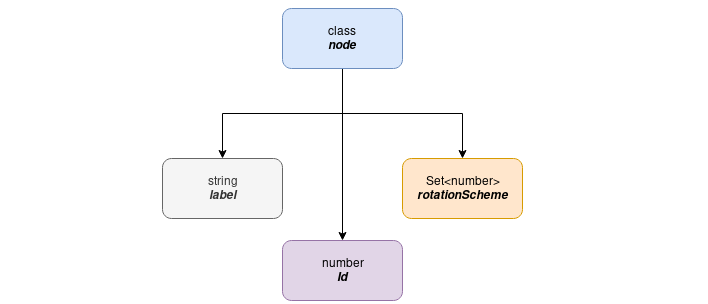
\includegraphics[width=1 \linewidth]{figure/nodeClass}
	\end{center}
	\caption{Oggetto nodo del underlying graph\label{fig:nodeClass}}
\end{figure}
blablalba
\begin{figure}[!htb]
	\begin{center}
		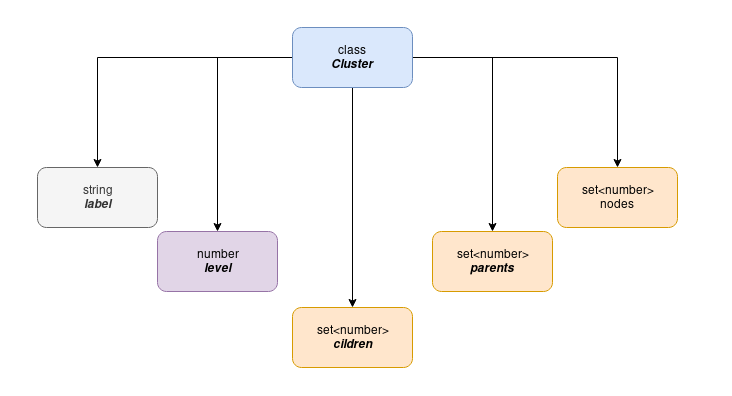
\includegraphics[width=1 \linewidth]{figure/clusterClass}
	\end{center}
	\caption{Oggetto cluster dell'inclusion Tree\label{fig:clusterClass}}
\end{figure}
blablalbablablalbablablalba
blablalbablablalbablablalba
blablalbablablalbablablalba
\begin{figure}[!htb]
	\begin{center}
		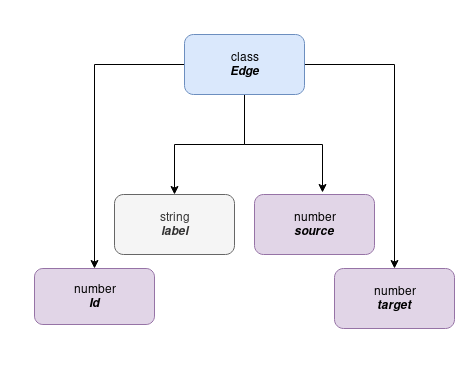
\includegraphics[width=1 \linewidth]{figure/edgeClass}
	\end{center}
	\caption{Oggetto arco dell'undelying graph\label{fig:edgeClass}}
\end{figure}

blablalbablablalbablablalbablablalba
blablalbablablalbablablalbablablalba



\section{Log-in ed inizializzazione}

\section{Graph-view}
\section{Tree-view}
\section{Console-view}

}
